\documentclass[aspectratio=169]{beamer}

%=========================================================
% Packages and Theme
%=========================================================

\usetheme{Madrid}

\usepackage[T1]{fontenc}
\usepackage{lmodern}
\usepackage{graphicx}
\usepackage{booktabs}
\usepackage{tikz}
\usetikzlibrary{positioning,arrows.meta,shapes.geometric,calc}
\usepackage{hyperref}
\usepackage{amsmath}

%=========================================================
% Colors
%=========================================================

\definecolor{CNUBlue}{RGB}{0,51,102}
\definecolor{CNUGold}{RGB}{181,136,52}
\definecolor{SoftGray}{RGB}{245,245,245}
\definecolor{DarkGray}{RGB}{65,65,65}

\setbeamercolor{structure}{fg=CNUBlue}
\setbeamercolor{title}{fg=white,bg=CNUBlue}
\setbeamercolor{frametitle}{fg=white,bg=CNUBlue}
\setbeamercolor{block title}{fg=white,bg=CNUBlue}
\setbeamercolor{block body}{bg=SoftGray,fg=black}

\setbeamertemplate{navigation symbols}{}

%=========================================================
% Convenience commands
%=========================================================

\newcommand{\ISO}{\textsc{ISO}}
\newcommand{\term}[1]{\textbf{#1}}

%=========================================================
% Title Information
%=========================================================

\title{The Institutional Semantic Observatory}
\subtitle{Engineering Information Ecosystems for Explainable AI}

\author{Edward Brash}

\institute{
School of Engineering and Computing\\
Christopher Newport University
}

\date{July 2026}

%=========================================================
% Document
%=========================================================

\begin{document}

%=========================================================
\begin{frame}
    \titlepage
\end{frame}

%=========================================================
\begin{frame}{The Usual AI Picture Is Too Simple}

\Large

Many people imagine an AI system as

\vspace{0.5cm}

\begin{center}
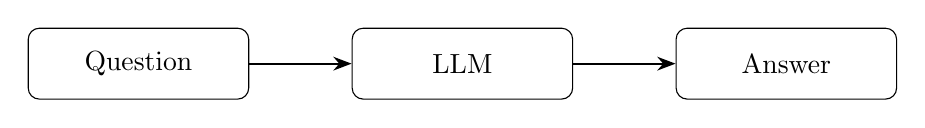
\begin{tikzpicture}[
node distance=1.3cm,
every node/.style={draw,rounded corners,minimum width=2.8cm,minimum height=0.9cm,align=center},
>=Stealth]
\node (q) {Question};
\node (m) [right=of q] {LLM};
\node (a) [right=of m] {Answer};
\draw[->,thick] (q)--(m);
\draw[->,thick] (m)--(a);
\end{tikzpicture}
\end{center}

\vspace{0.6cm}

That picture is useful, but incomplete.

\vspace{0.4cm}

For institutional reasoning, the hard part is often not the final answer.
It is constructing the information environment in which reliable reasoning becomes possible.

\end{frame}

%=========================================================
\begin{frame}{What ISO Is}

\Large

\begin{block}{Institutional Semantic Observatory}
\ISO{} is an architecture for constructing, maintaining, observing, and reasoning over institutional knowledge.
\end{block}

\vspace{0.6cm}

It is not simply a chatbot and it is not simply a RAG system.

\vspace{0.4cm}

It is a measurement and reasoning framework for institutional information ecosystems.

\end{frame}

%=========================================================
\begin{frame}{The Core Question}

\Large

\begin{block}{Human reasoning benchmark}
Given this information corpus, what would an intelligent human using appropriate reasoning skills conclude?
\end{block}

\vspace{0.7cm}

The goal is for the system to approximate that process:

\begin{enumerate}
\item identify relevant evidence,
\item organize it coherently,
\item reason transparently,
\item expose uncertainty,
\item and support a defensible human decision.
\end{enumerate}

\end{frame}

%=========================================================
\begin{frame}{Why Human Reasoning Alone Is Not Enough}

\begin{columns}[T]

\column{0.48\textwidth}

\begin{block}{Scale}
An expert may need evidence scattered across thousands of documents.

\vspace{0.2cm}

Even an excellent dean cannot read the entire corpus for every strategic question.
\end{block}

\column{0.48\textwidth}

\begin{block}{Recall}
The right evidence may be hidden in ten documents among fifteen thousand.

\vspace{0.2cm}

The expert may reason well, but never see the crucial source.
\end{block}

\end{columns}

\vspace{0.7cm}

\begin{center}
\Large
Human reasoning is often not the bottleneck.\\[0.2cm]
\textbf{Evidence discovery is.}
\end{center}

\end{frame}

%=========================================================
\begin{frame}{ISO Reframes the Bottleneck}

\begin{center}
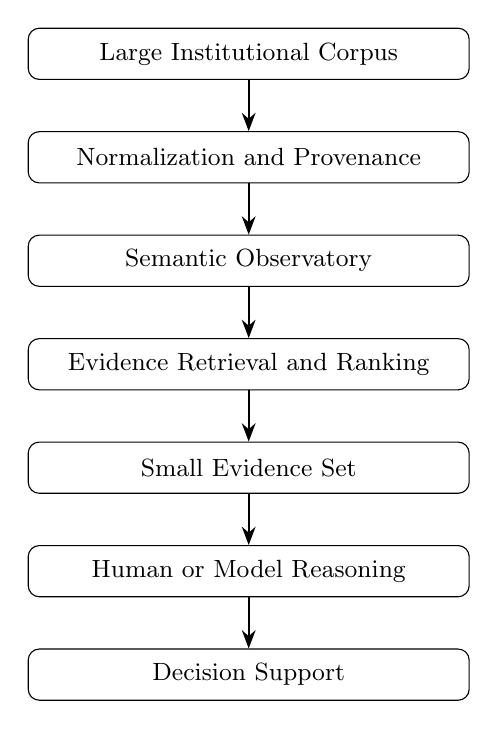
\begin{tikzpicture}[
node distance=0.65cm,
every node/.style={draw,rounded corners,minimum width=5.6cm,minimum height=0.65cm,align=center,font=\small},
>=Stealth]
\node (corpus) {Large Institutional Corpus};
\node (norm) [below=of corpus] {Normalization and Provenance};
\node (obs) [below=of norm] {Semantic Observatory};
\node (retr) [below=of obs] {Evidence Retrieval and Ranking};
\node (ev) [below=of retr] {Small Evidence Set};
\node (reason) [below=of ev] {Human or Model Reasoning};
\node (brief) [below=of reason] {Decision Support};
\draw[->,thick] (corpus)--(norm);
\draw[->,thick] (norm)--(obs);
\draw[->,thick] (obs)--(retr);
\draw[->,thick] (retr)--(ev);
\draw[->,thick] (ev)--(reason);
\draw[->,thick] (reason)--(brief);
\end{tikzpicture}
\end{center}

\end{frame}

%=========================================================
\begin{frame}{Two Philosophies of AI System Design}

\small

\begin{table}
\begin{tabular}{p{0.45\textwidth}p{0.45\textwidth}}
\toprule
\textbf{Conventional AI framing} & \textbf{ISO framing} \\
\midrule
Intelligence resides primarily in the model. & Intelligence emerges from the interaction between the reasoning engine and the information environment. \\
\addlinespace
Build a very capable model, then prevent it from doing bad things. & Build an information environment in which good reasoning is the natural outcome. \\
\addlinespace
Guardrails constrain the actor. & Guardrails engineer the environment. \\
\addlinespace
Better model $\rightarrow$ better answer. & Better ecosystem $\rightarrow$ better evidence $\rightarrow$ better reasoning. \\
\bottomrule
\end{tabular}
\end{table}

\vspace{0.35cm}

\begin{center}
\Large
\textbf{The most effective guardrail is a well-engineered information environment.}
\end{center}

\end{frame}

%=========================================================
\begin{frame}{Guardrails: Where Do They Live?}

\begin{center}
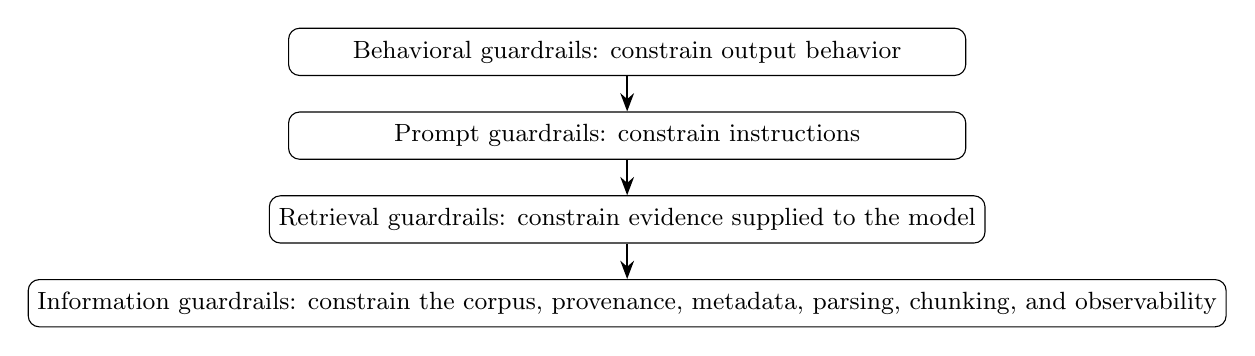
\begin{tikzpicture}[
node distance=0.45cm,
every node/.style={draw,rounded corners,minimum width=8.6cm,minimum height=0.6cm,align=center,font=\small},
>=Stealth]
\node (behavior) {Behavioral guardrails: constrain output behavior};
\node (prompt) [below=of behavior] {Prompt guardrails: constrain instructions};
\node (retrieval) [below=of prompt] {Retrieval guardrails: constrain evidence supplied to the model};
\node (info) [below=of retrieval] {Information guardrails: constrain the corpus, provenance, metadata, parsing, chunking, and observability};
\draw[->,thick] (behavior)--(prompt);
\draw[->,thick] (prompt)--(retrieval);
\draw[->,thick] (retrieval)--(info);
\end{tikzpicture}
\end{center}

\vspace{0.45cm}

\ISO{} places many of the most important guardrails below the LLM, where they can be explicit, inspectable, and auditable.

\end{frame}

%=========================================================
\begin{frame}{Knowledge Objects Store Facts}

\Large

\begin{block}{Knowledge objects store facts.}
Documents, metadata, source paths, timestamps, parser information, chunk boundaries, and provenance.
\end{block}

\vspace{0.55cm}

\begin{block}{Services derive meaning.}
Retrieval, ranking, synthesis, decision briefs, observatory metrics, and scenario analysis.
\end{block}

\vspace{0.55cm}

This separation keeps the evidence layer stable while allowing multiple reasoning services to operate over it.

\end{frame}

%=========================================================
\begin{frame}{The ISO Pipeline}

\centering

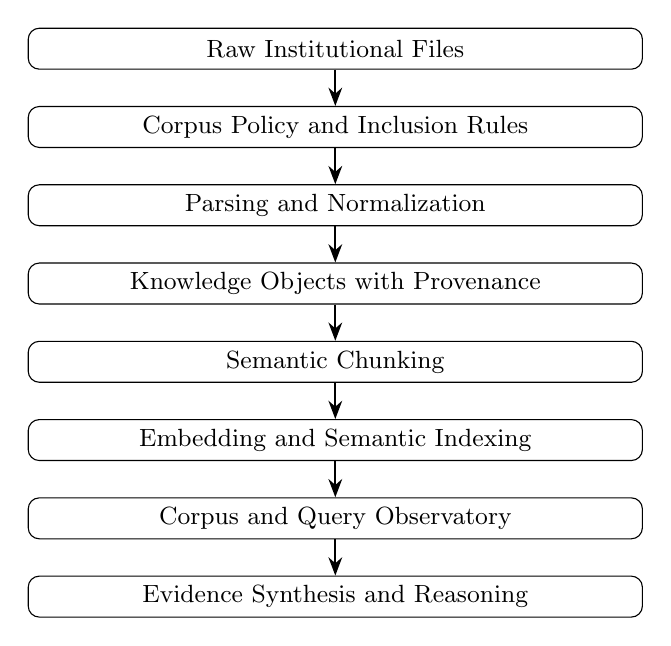
\begin{tikzpicture}[
node distance=0.46cm,
every node/.style={draw,rounded corners,minimum width=7.8cm,minimum height=0.52cm,align=center,font=\small},
>=Stealth]
\node (raw) {Raw Institutional Files};
\node (policy) [below=of raw] {Corpus Policy and Inclusion Rules};
\node (parse) [below=of policy] {Parsing and Normalization};
\node (ko) [below=of parse] {Knowledge Objects with Provenance};
\node (chunk) [below=of ko] {Semantic Chunking};
\node (embed) [below=of chunk] {Embedding and Semantic Indexing};
\node (obs) [below=of embed] {Corpus and Query Observatory};
\node (reason) [below=of obs] {Evidence Synthesis and Reasoning};
\draw[->,thick] (raw)--(policy);
\draw[->,thick] (policy)--(parse);
\draw[->,thick] (parse)--(ko);
\draw[->,thick] (ko)--(chunk);
\draw[->,thick] (chunk)--(embed);
\draw[->,thick] (embed)--(obs);
\draw[->,thick] (obs)--(reason);
\end{tikzpicture}

\end{frame}

%=========================================================
\begin{frame}{The Semantic Ecosystem}

\begin{block}{Working metaphor}
An institutional corpus behaves less like a filing cabinet and more like an ecosystem.
\end{block}

\vspace{0.4cm}

Healthy semantic ecosystems have

\begin{itemize}
\item diversity,
\item balance,
\item provenance,
\item redundancy without pathological duplication,
\item observable structure,
\item and resilience to noise.
\end{itemize}

\vspace{0.3cm}

Unhealthy ecosystems contain corrupted documents, dominant outliers, stale knowledge, duplicated artifacts, and isolated semantic islands.

\end{frame}

%=========================================================
\begin{frame}{The Observatory Is Not Decorative}

\Large

\begin{block}{Analogy}
A physicist would not trust a detector analysis without detector monitoring, calibration checks, acceptance studies, and quality plots.
\end{block}

\vspace{0.6cm}

Likewise, we should not trust AI-assisted institutional reasoning without instrumentation of the underlying semantic environment.

\vspace{0.6cm}

\begin{center}
\textbf{The observatory is part of the scientific instrument.}
\end{center}

\end{frame}

%=========================================================
\begin{frame}{Corpus Observatory: Global Health}

\begin{columns}[T]
\column{0.47\textwidth}

\begin{block}{Global metrics}
\begin{itemize}
\item document count
\item chunk count
\item parser distribution
\item file-type distribution
\item largest documents
\item chunk dominance
\item Gini coefficient
\end{itemize}
\end{block}

\column{0.47\textwidth}

\begin{block}{Why it matters}
\begin{itemize}
\item detects corrupted documents
\item reveals duplicated material
\item identifies dominant sources
\item monitors pipeline health
\item makes semantic risk visible
\end{itemize}
\end{block}

\end{columns}

\end{frame}

%=========================================================
\begin{frame}{Local Information Density}

\Large

A question lives somewhere in semantic space.

\vspace{0.5cm}

Some regions are densely supported by institutional evidence.

\vspace{0.3cm}

Other regions are sparse.

\vspace{0.7cm}

\begin{block}{Key idea}
Hallucination risk is often not merely a model problem. It may indicate low local information density near the query.
\end{block}

\end{frame}

%=========================================================
\begin{frame}{From Corpus Observatory to Query Observatory}

\begin{columns}[T]

\column{0.48\textwidth}

\begin{block}{Corpus Observatory}
Measures the global health of the information ecosystem.

\begin{itemize}
\item corpus size
\item dominance
\item parser health
\item distribution
\item outliers
\end{itemize}
\end{block}

\column{0.48\textwidth}

\begin{block}{Query Observatory}
Measures how well-supported a particular question is.

\begin{itemize}
\item local information density
\item evidence diversity
\item provenance quality
\item retrieval stability
\item evidence completeness
\end{itemize}
\end{block}

\end{columns}

\end{frame}

%=========================================================
\begin{frame}{A Query Diagnostic Panel}

\small

\begin{block}{Question}
What resources would be required to launch a Mechanical Engineering major?
\end{block}

\vspace{0.35cm}

\begin{tabular}{p{0.45\textwidth}p{0.38\textwidth}r}
Local information density & \rule{3.6cm}{0.15cm} & 9.4/10 \\
Evidence diversity & \rule{3.2cm}{0.15cm} & 8.8/10 \\
Provenance quality & \rule{3.4cm}{0.15cm} & 9.1/10 \\
Retrieval stability & \rule{3.1cm}{0.15cm} & 8.4/10 \\
Evidence completeness & \rule{3.0cm}{0.15cm} & 8.1/10 \\
\end{tabular}

\vspace{0.5cm}

\begin{center}
\Large
Expected reasoning reliability: \textbf{High}
\end{center}

\end{frame}

%=========================================================
\begin{frame}{When the Evidence Is Not Enough}

\small

\begin{block}{Question}
Should CNU eliminate the French major?
\end{block}

\vspace{0.3cm}

A good decision-support system should not invent enrollment, budget, faculty, or strategic evidence that is not present.

\vspace{0.4cm}

Instead it should report

\begin{itemize}
\item what evidence was retrieved,
\item what conclusions that evidence supports,
\item what conclusions it does not support,
\item and what information is missing.
\end{itemize}

\vspace{0.3cm}

\begin{center}
\Large
\textbf{Epistemic humility is a feature, not a failure.}
\end{center}

\end{frame}

%=========================================================
\begin{frame}{Diagnosing Hallucinations}

\small

Not all hallucinations have the same cause.

\vspace{0.3cm}

\begin{table}
\begin{tabular}{p{0.3\textwidth}p{0.55\textwidth}}
\toprule
\textbf{Failure mode} & \textbf{ISO response} \\
\midrule
Missing evidence & Improve corpus coverage; report insufficiency. \\
Poor retrieval & Improve retrieval, reranking, benchmarks, and diagnostics. \\
Ambiguous or conflicting evidence & Surface disagreement and uncertainty. \\
Reasoning error & Improve prompts, models, validation, or human review. \\
\bottomrule
\end{tabular}
\end{table}

\vspace{0.35cm}

The symptom may be one wrong answer; the causes live at different layers of the system.

\end{frame}

%=========================================================
\begin{frame}{Evidence Quality Is Not Model Confidence}

\Large

A language model may sound confident even when the evidence is weak.

\vspace{0.55cm}

\begin{block}{ISO question}
How well-supported is this question by the available institutional evidence?
\end{block}

\vspace{0.55cm}

That is not the same as asking whether the model produced fluent text.

\vspace{0.4cm}

The observatory should measure evidence support before the final reasoning step.

\end{frame}

%=========================================================
\begin{frame}{From RAG to Institutional Reasoning}

\begin{center}
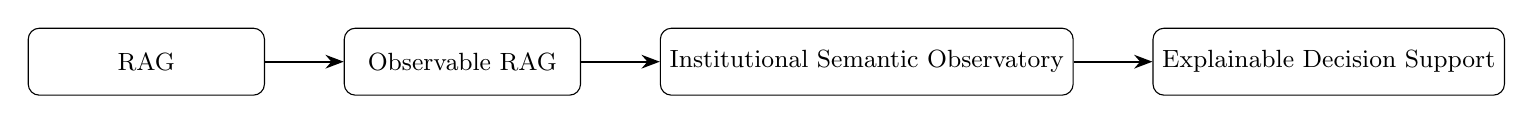
\begin{tikzpicture}[
node distance=1.0cm,
every node/.style={draw,rounded corners,minimum width=3.0cm,minimum height=0.85cm,align=center,font=\small},
>=Stealth]
\node (rag) {RAG};
\node (obs) [right=of rag] {Observable RAG};
\node (iso) [right=of obs] {Institutional Semantic Observatory};
\node (reason) [right=of iso] {Explainable Decision Support};
\draw[->,thick] (rag)--(obs);
\draw[->,thick] (obs)--(iso);
\draw[->,thick] (iso)--(reason);
\end{tikzpicture}
\end{center}

\vspace{0.7cm}

The progression is not primarily about larger models.

\vspace{0.3cm}

It is about better instrumentation of the information environment.

\end{frame}

%=========================================================
\begin{frame}{Research Questions}

\small

\begin{itemize}
\item Does local information density correlate with answer quality?
\item Does retrieval stability predict benchmark performance?
\item Does evidence diversity reduce reasoning errors?
\item Can provenance quality predict user trust?
\item Can evidence completeness identify when a system should refuse to recommend?
\item Can query-level observatory metrics become calibrated reliability estimates?
\end{itemize}

\vspace{0.4cm}

These are empirical questions that can be tested inside a real institutional knowledge system.

\end{frame}

%=========================================================
\begin{frame}{The Technical Thesis}

\Large

\begin{block}{Central claim}
Reliable reasoning is not simply a property of the reasoning engine.
\end{block}

\vspace{0.5cm}

It is an emergent property of

\begin{itemize}
\item a well-engineered corpus,
\item explicit provenance,
\item observable retrieval,
\item evidence diagnostics,
\item and human-governed interpretation.
\end{itemize}

\end{frame}

%=========================================================
\begin{frame}{Closing}

\centering

\vspace{0.6cm}

{\LARGE ISO is not mainly about making a model smarter.}

\vspace{1cm}

{\LARGE It is about building the information environment in which good reasoning becomes possible.}

\vfill

{\large Thank you.}

\end{frame}

%=========================================================
\end{document}
